% ================= SEKCJA 7 =================
\section{Makiety i interfejs użytkownika}

Interfejs użytkownika systemu \texttt{WorkFlow} został zaprojektowany z myślą o pracy administracyjnej wykonywanej z poziomu przeglądarki internetowej. Głównym założeniem było przygotowanie widoków, które pozwalają szybko przejść do najważniejszych modułów systemu: pracowników, zakładów, projektów, czasu pracy, certyfikatów, dokumentów, nieobecności oraz rozliczeń.

W początkowej fazie projektu przygotowano makiety interfejsu, które pozwoliły określić ogólny układ aplikacji oraz rozmieszczenie najważniejszych informacji. W późniejszej implementacji część widoków została dostosowana do aktualnego zakresu funkcjonalnego systemu oraz do zastosowanego stosu technologicznego.

\subsection{Założenia projektowe interfejsu}

Podczas projektowania interfejsu przyjęto następujące założenia:
\begin{itemize}
    \item system powinien posiadać czytelną nawigację boczną,
    \item główne moduły powinny być dostępne z poziomu panelu użytkownika,
    \item widoki powinny być spójne pod względem układu formularzy, tabel i przycisków,
    \item dane powinny być możliwe do filtrowania i wyszukiwania,
    \item formularze powinny wskazywać wymagane dane oraz obsługiwać błędy walidacji,
    \item interfejs powinien poprawnie działać w trybie jasnym i ciemnym,
    \item użytkownik powinien widzieć tylko te elementy, do których ma dostęp zgodnie ze swoją rolą.
\end{itemize}

Aplikacja ma charakter panelu administracyjnego. Z tego względu najważniejsza była czytelność danych, łatwość przeglądania tabel oraz możliwość szybkiego przejścia do szczegółów rekordu.

\subsection{Pulpit główny}

Pulpit główny stanowi pierwszy ekran po zalogowaniu użytkownika. Jego zadaniem jest zebranie najważniejszych informacji oraz zapewnienie szybkiego dostępu do modułów systemu.

\begin{figure}[H]
    \centering
    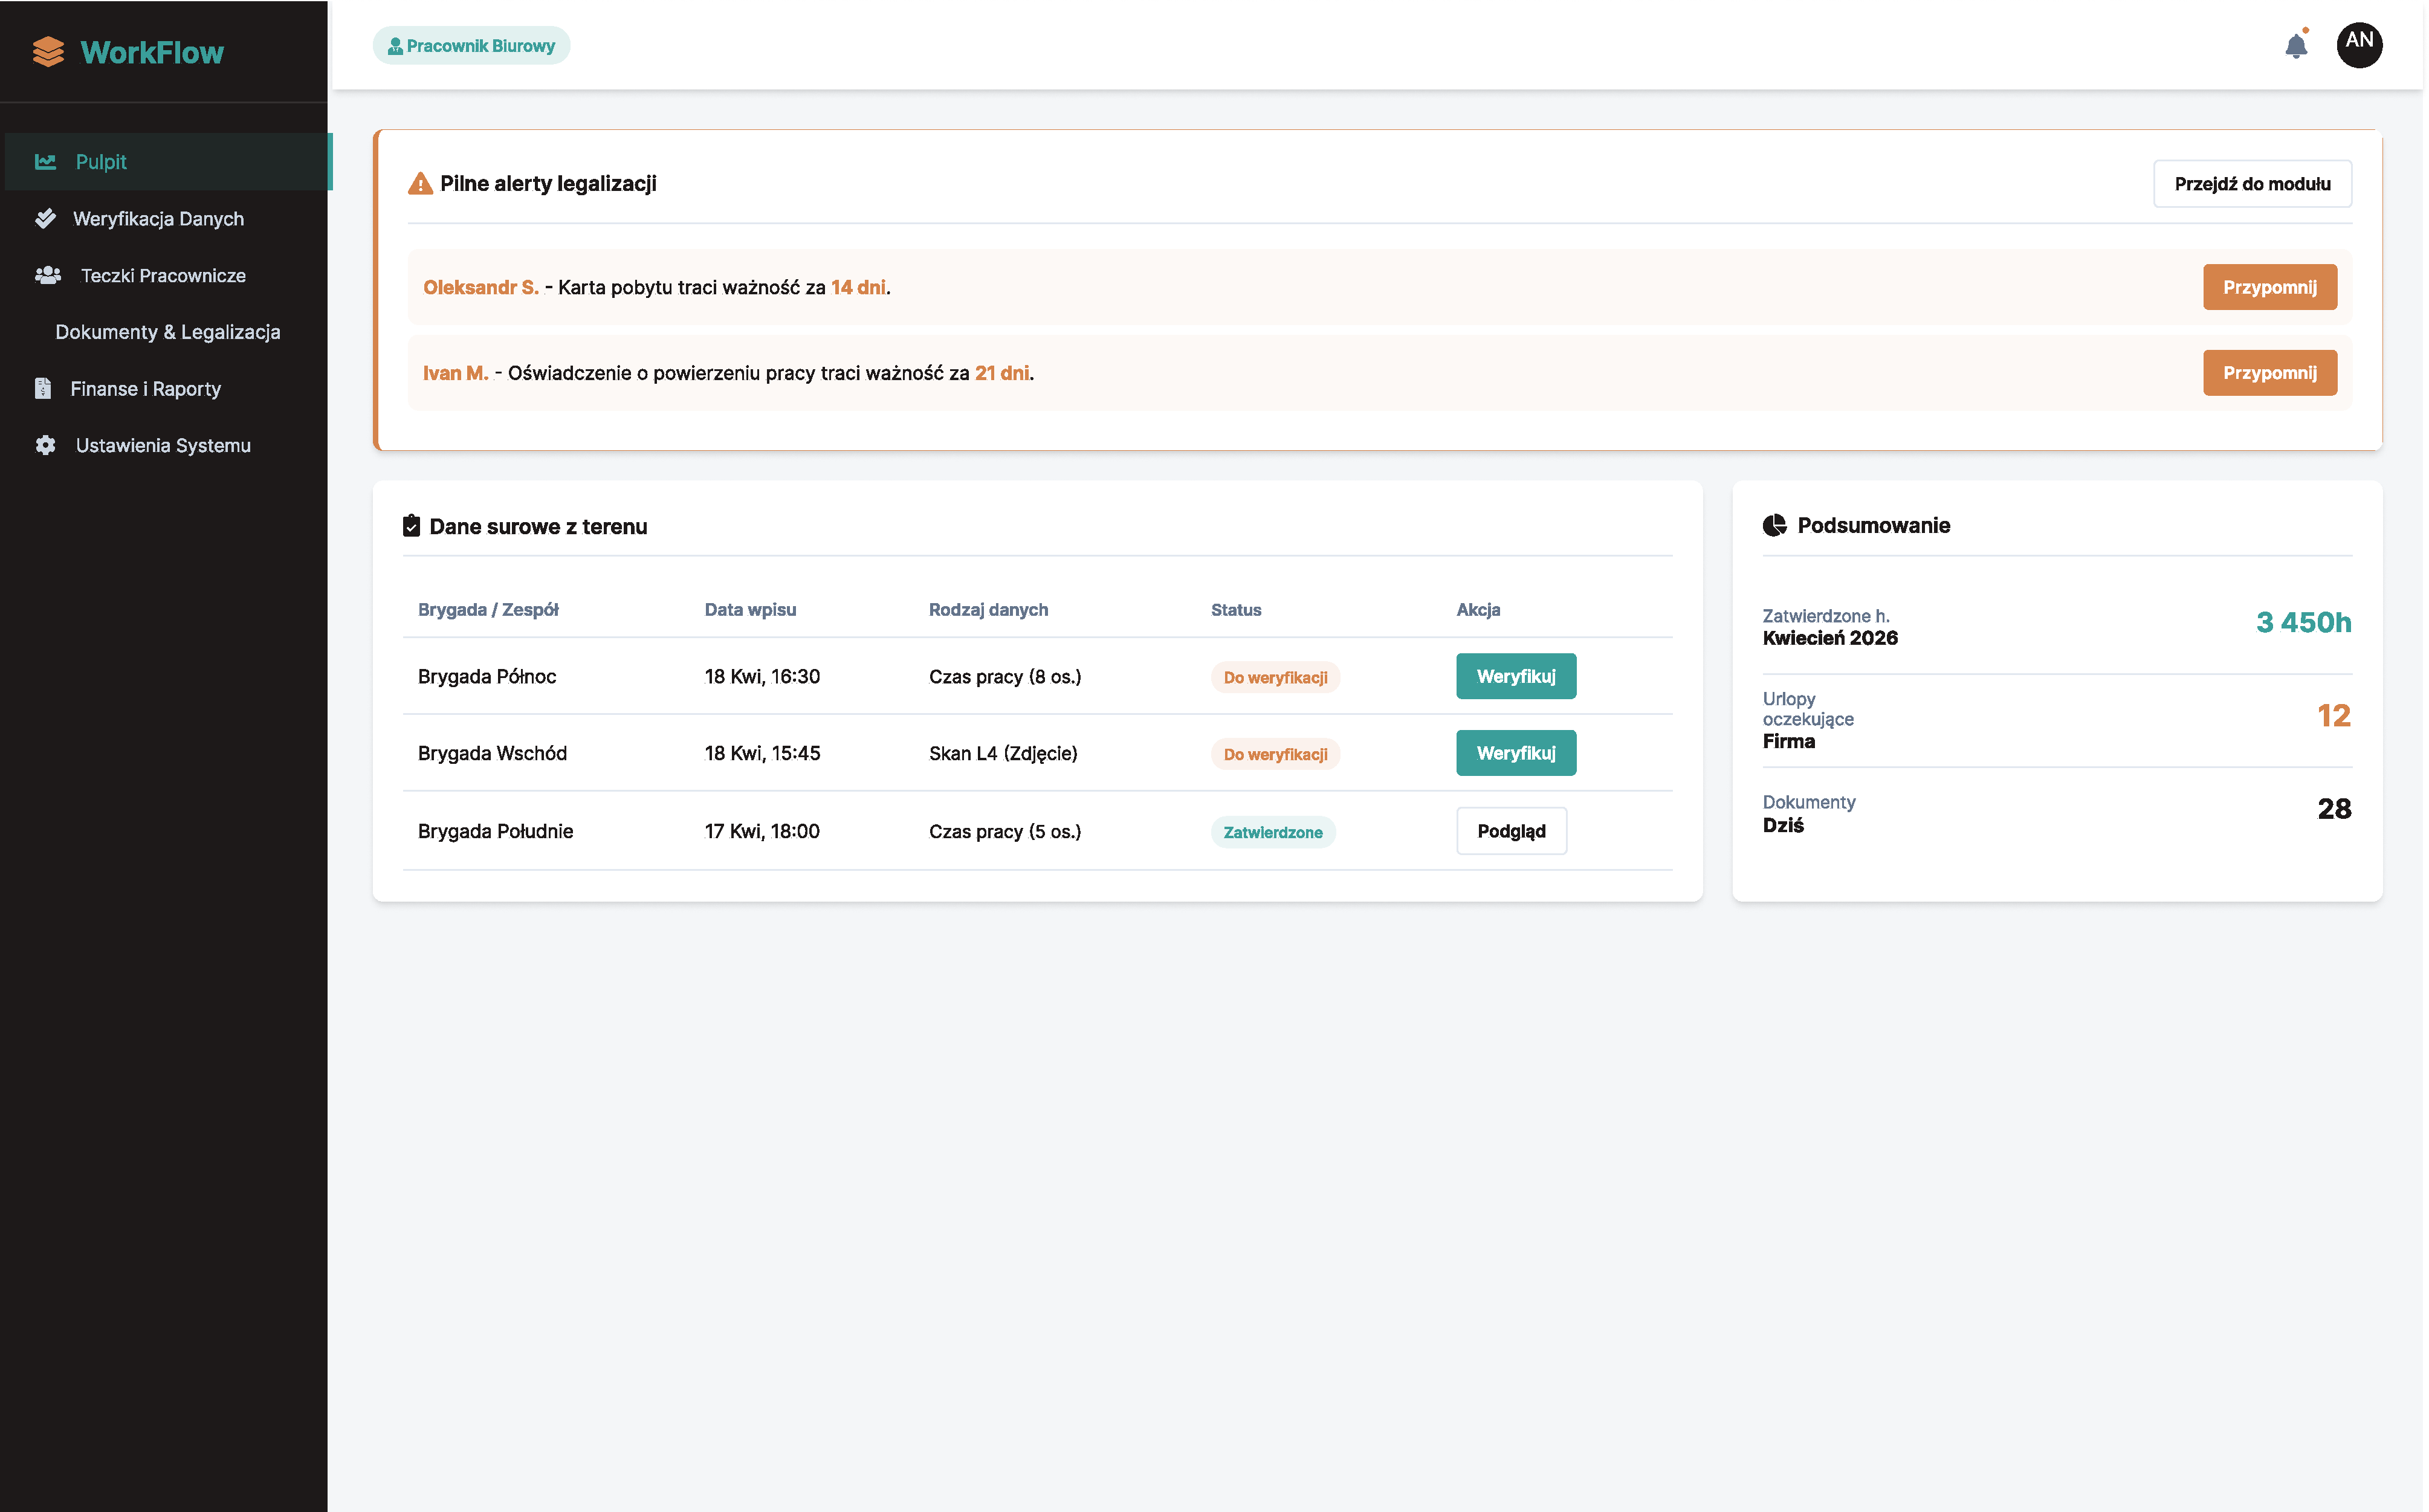
\includegraphics[width=0.95\textwidth]{rys/1920w.pdf}
    \caption{Widok desktopowy -- pulpit główny systemu \texttt{WorkFlow}}
    \label{fig:figma_dashboard_desktop}
\end{figure}

\begin{figure}[H]
    \centering
    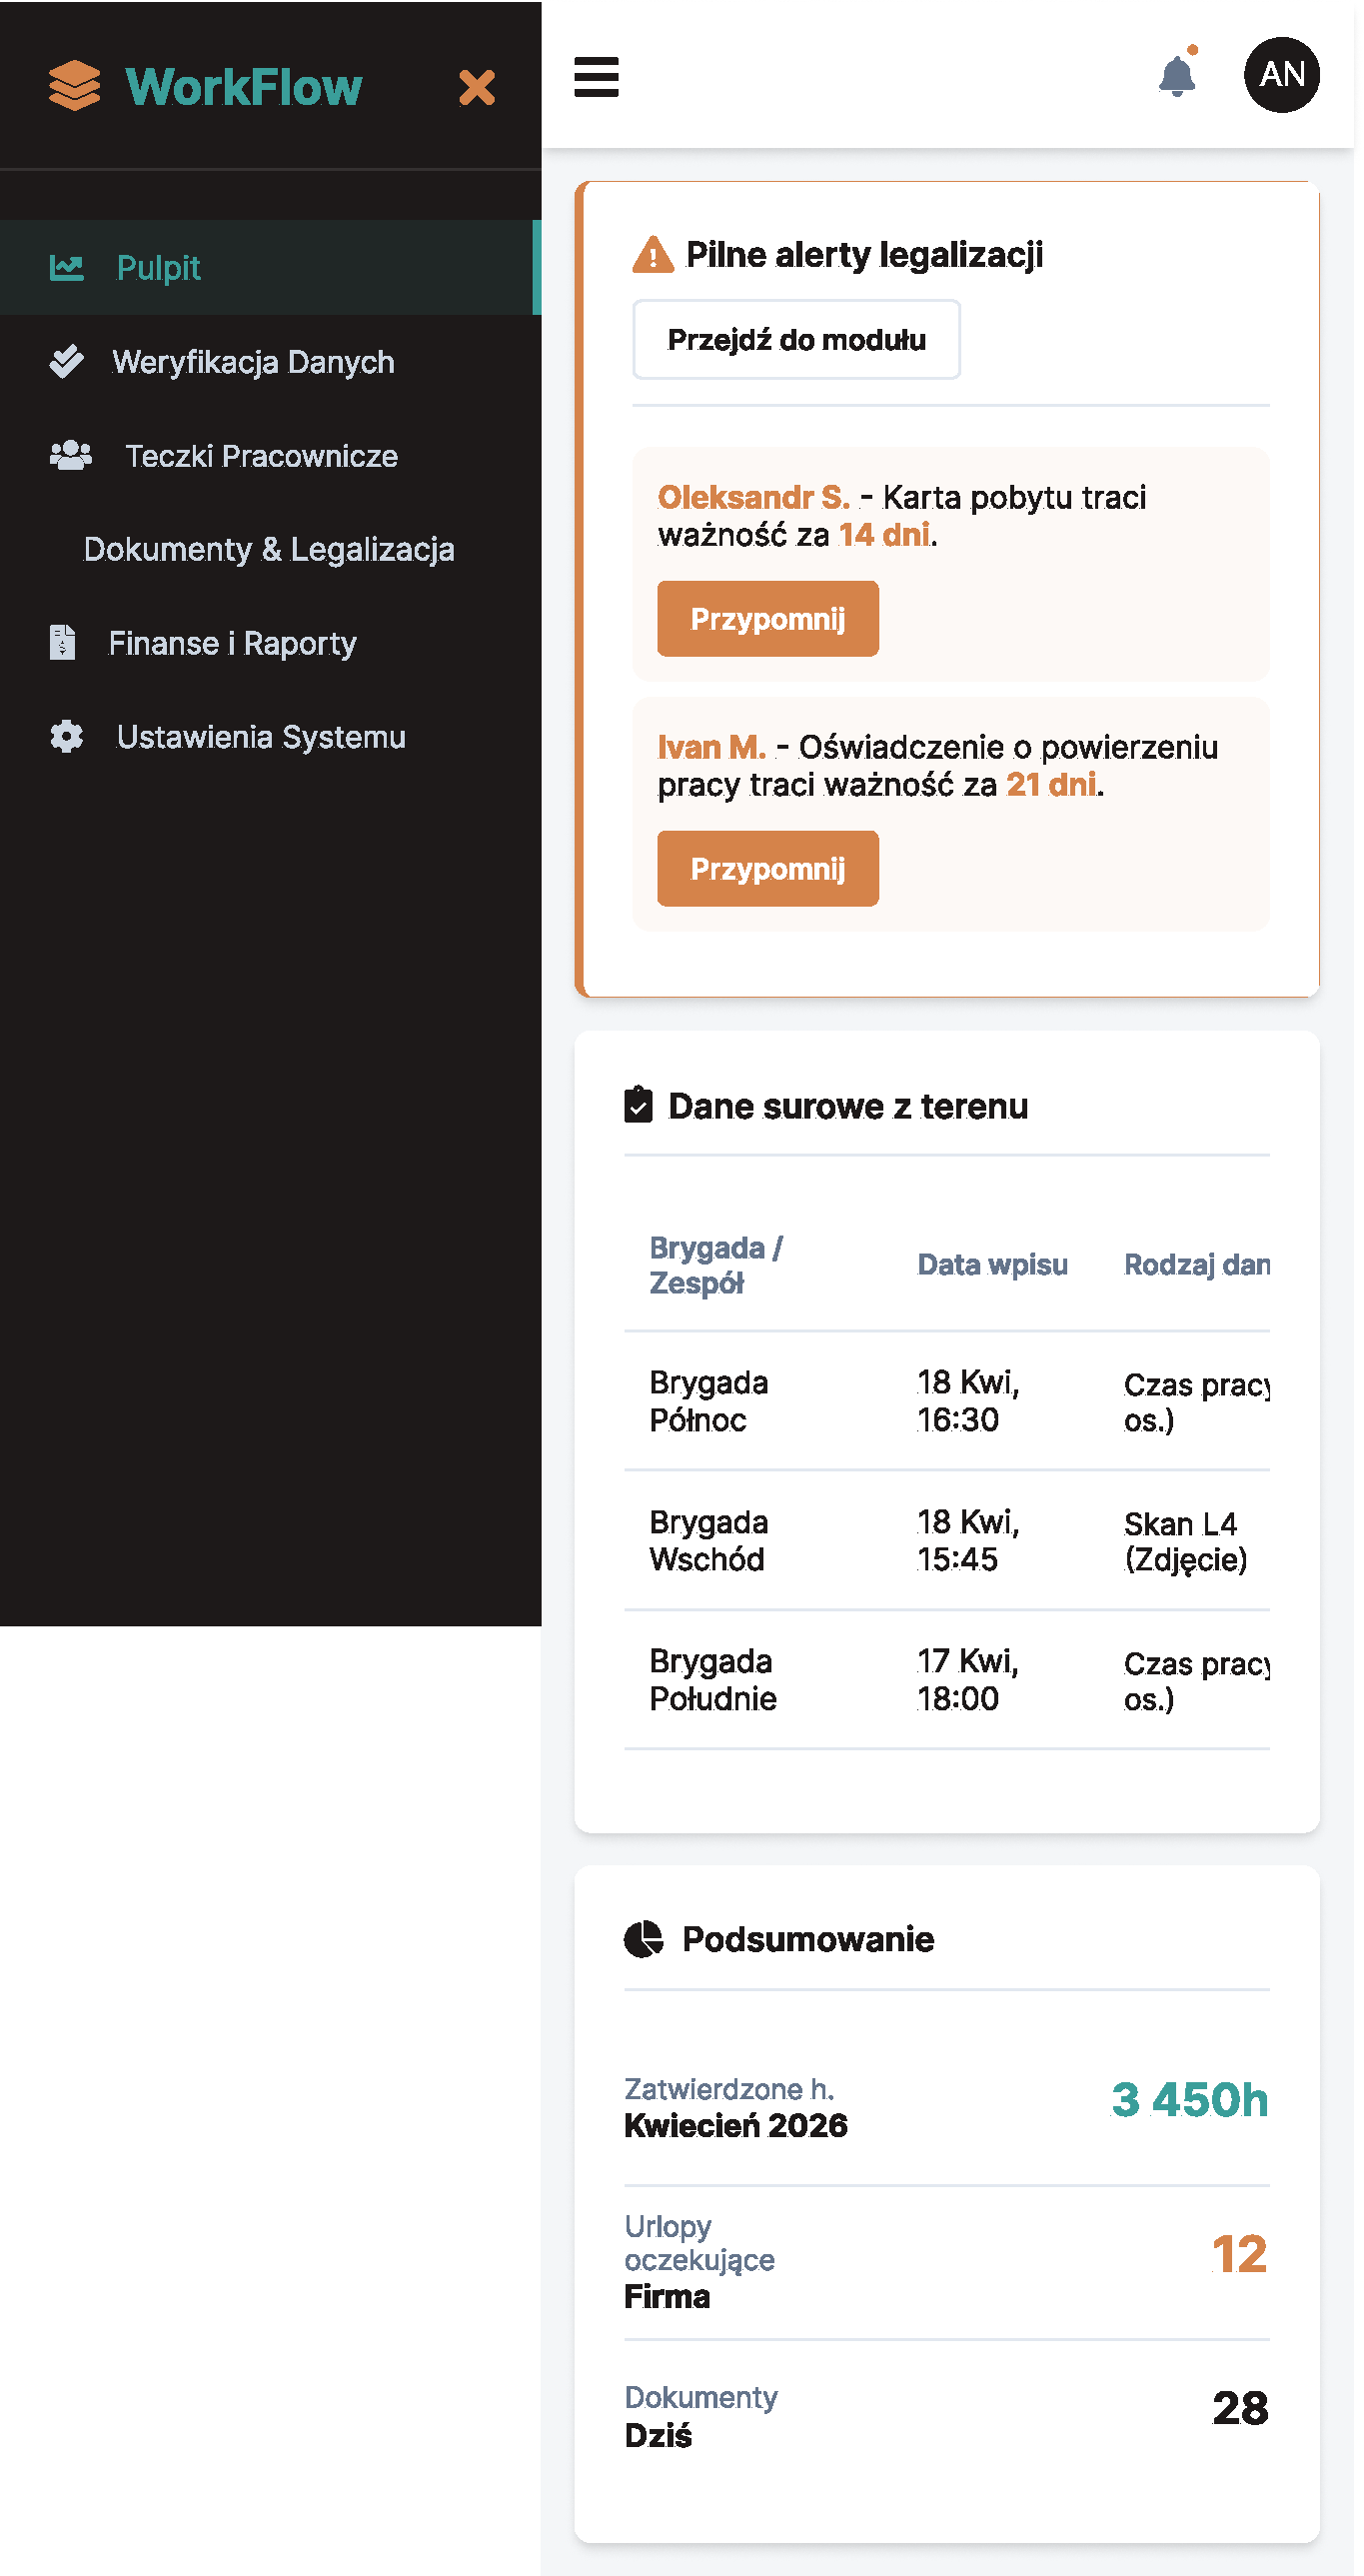
\includegraphics[width=0.35\textwidth]{rys/390w.pdf}
    \caption{Widok mobilny -- pulpit główny systemu \texttt{WorkFlow}}
    \label{fig:figma_dashboard_mobile}
\end{figure}

\textbf{Najważniejsze elementy pulpitu:}
\begin{itemize}
    \item \textbf{Nawigacja do modułów} -- użytkownik może przejść do widoków pracowników, zakładów, projektów, czasu pracy, certyfikatów i rozliczeń.
    \item \textbf{Kontekst zakładu} -- system uwzględnia zakład aktywny dla użytkownika, co pozwala ograniczyć zakres prezentowanych danych.
    \item \textbf{Podsumowania} -- widok może prezentować skrócone informacje dotyczące pracowników, projektów, certyfikatów lub czasu pracy.
    \item \textbf{Dostęp zależny od roli} -- zakres widocznych elementów zależy od tego, czy użytkownik pełni rolę administratora, HR, księgowości, brygadzisty lub inną rolę systemową.
\end{itemize}

Pulpit główny nie jest samodzielnym modułem biznesowym. Pełni rolę punktu startowego, który pozwala użytkownikowi przejść do dalszych obszarów systemu.

\subsection{Profil pracownika}

Profil pracownika jest jednym z najważniejszych widoków systemu. Łączy w jednym miejscu dane podstawowe pracownika oraz informacje powiązane z innymi modułami.

\begin{figure}[H]
    \centering
    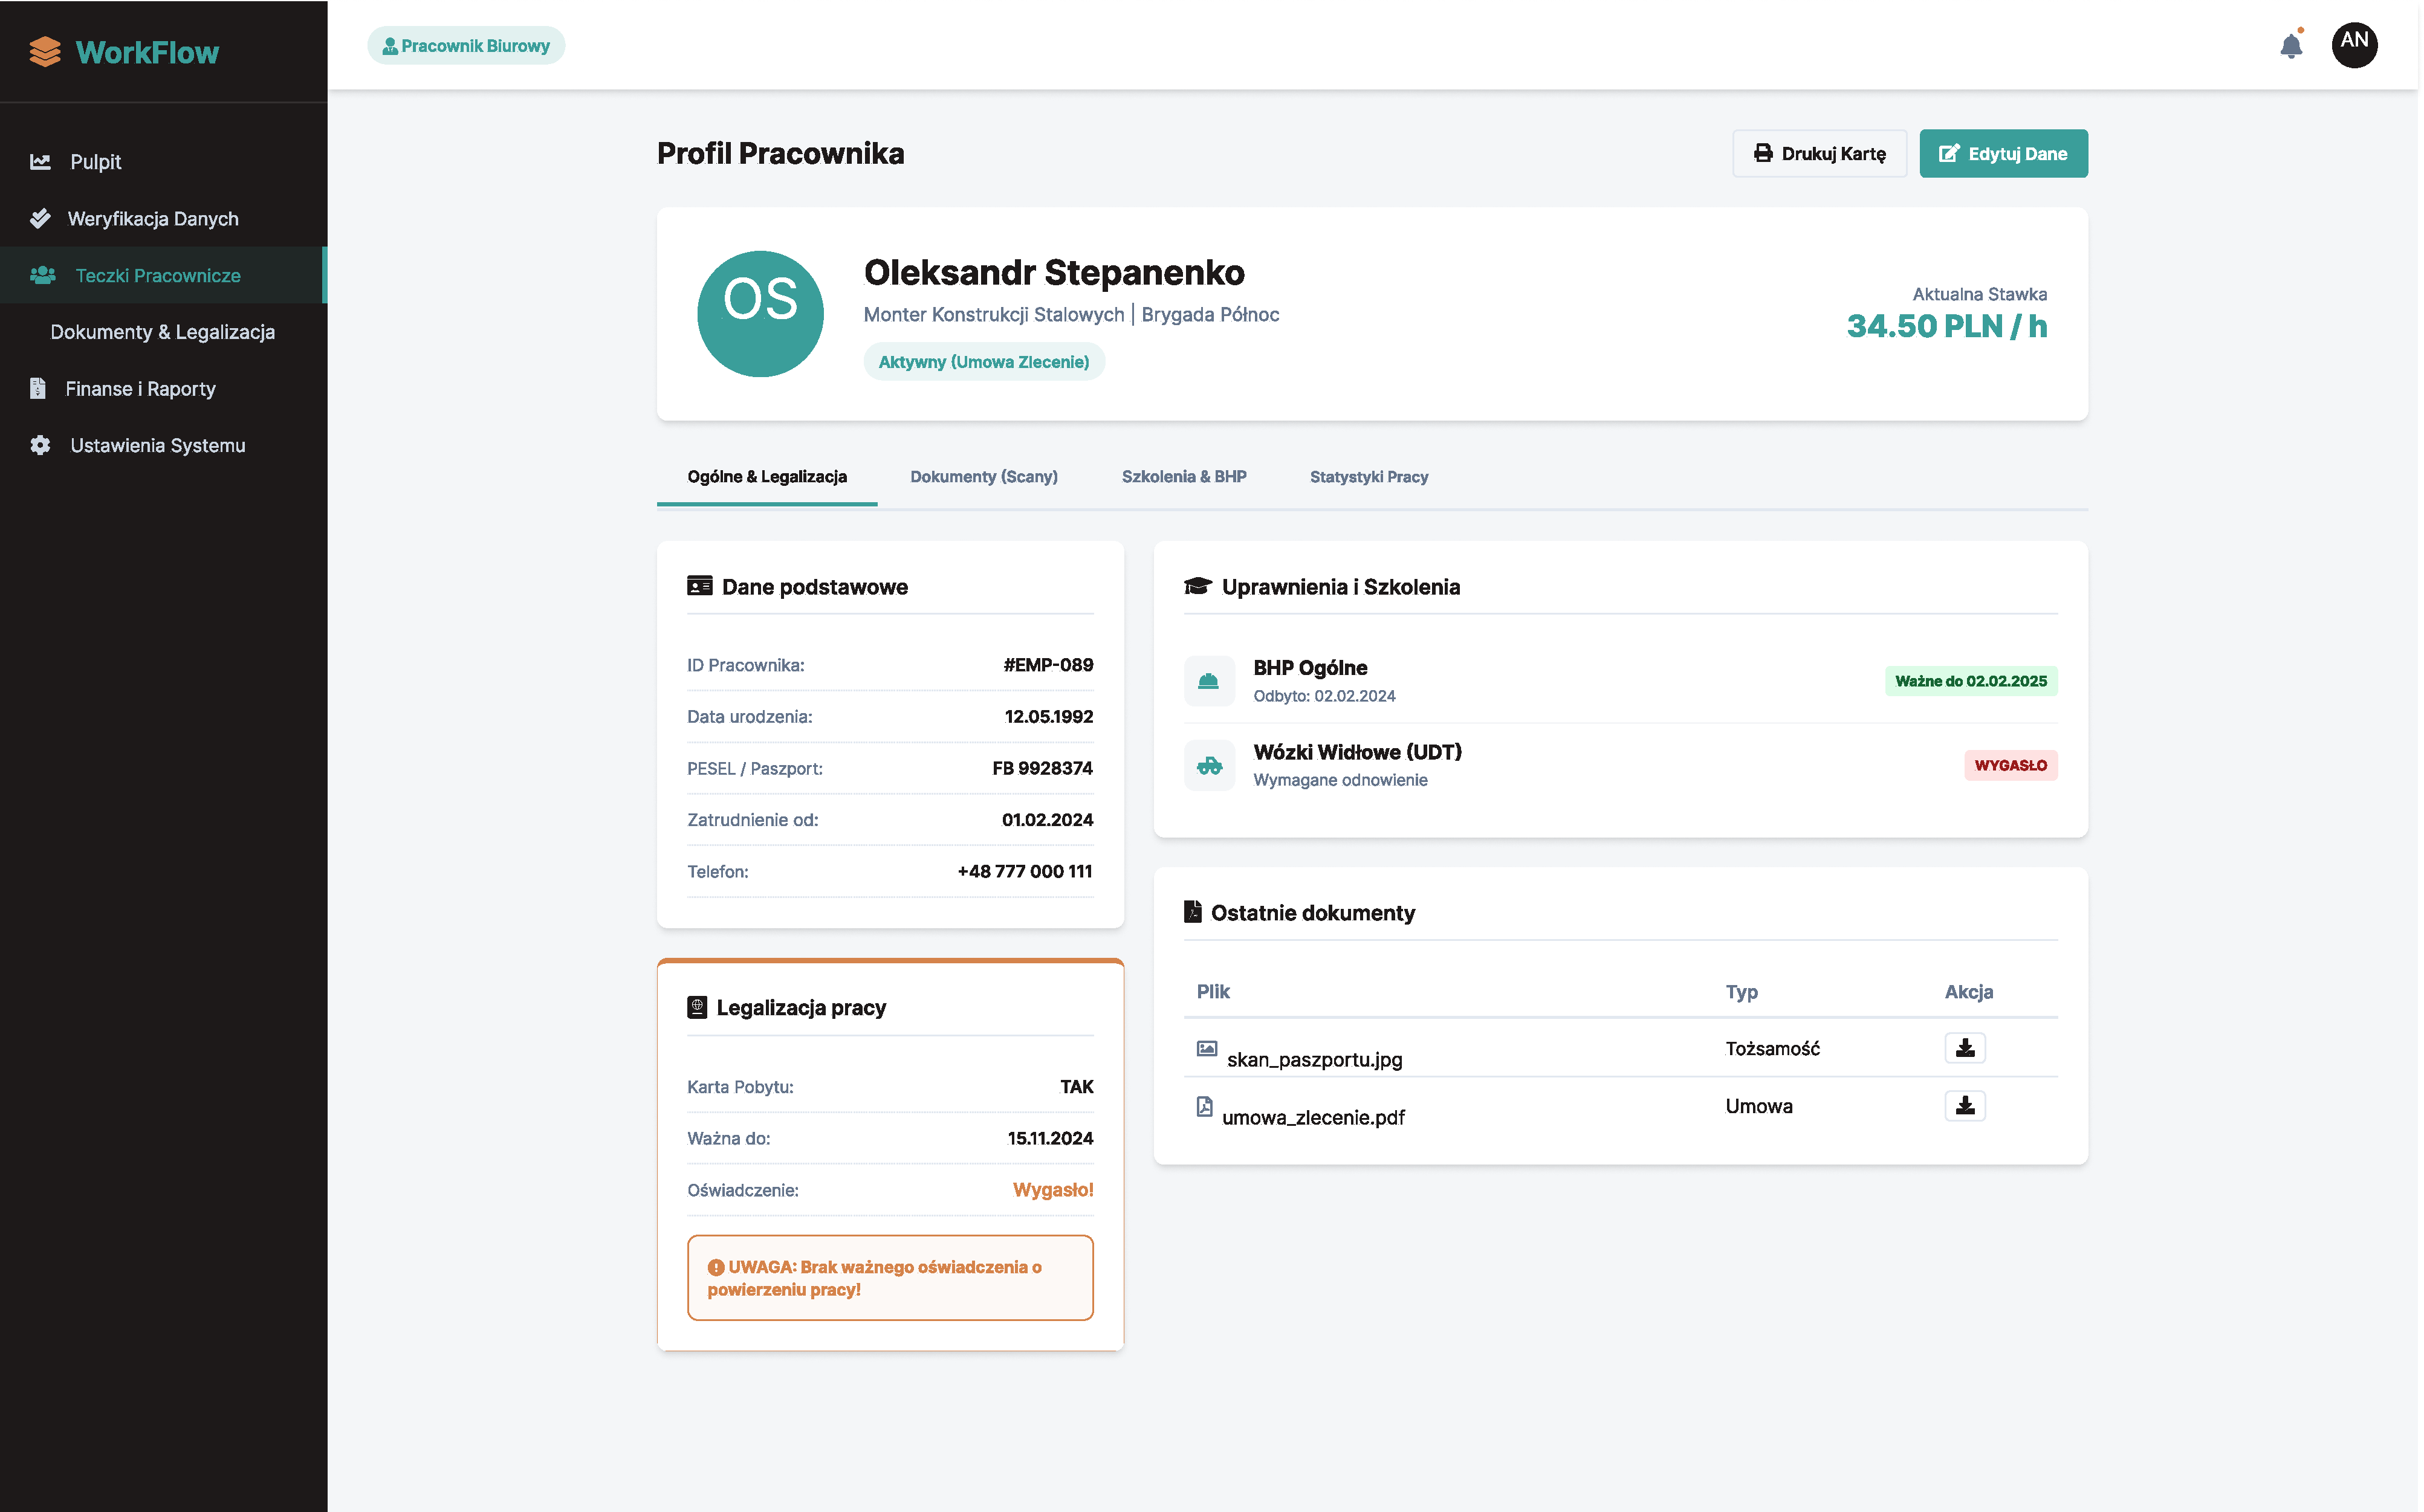
\includegraphics[width=0.95\textwidth]{rys/1920w_panel.pdf}
    \caption{Widok desktopowy -- profil pracownika}
    \label{fig:figma_profile_desktop}
\end{figure}

\begin{figure}[H]
    \centering
    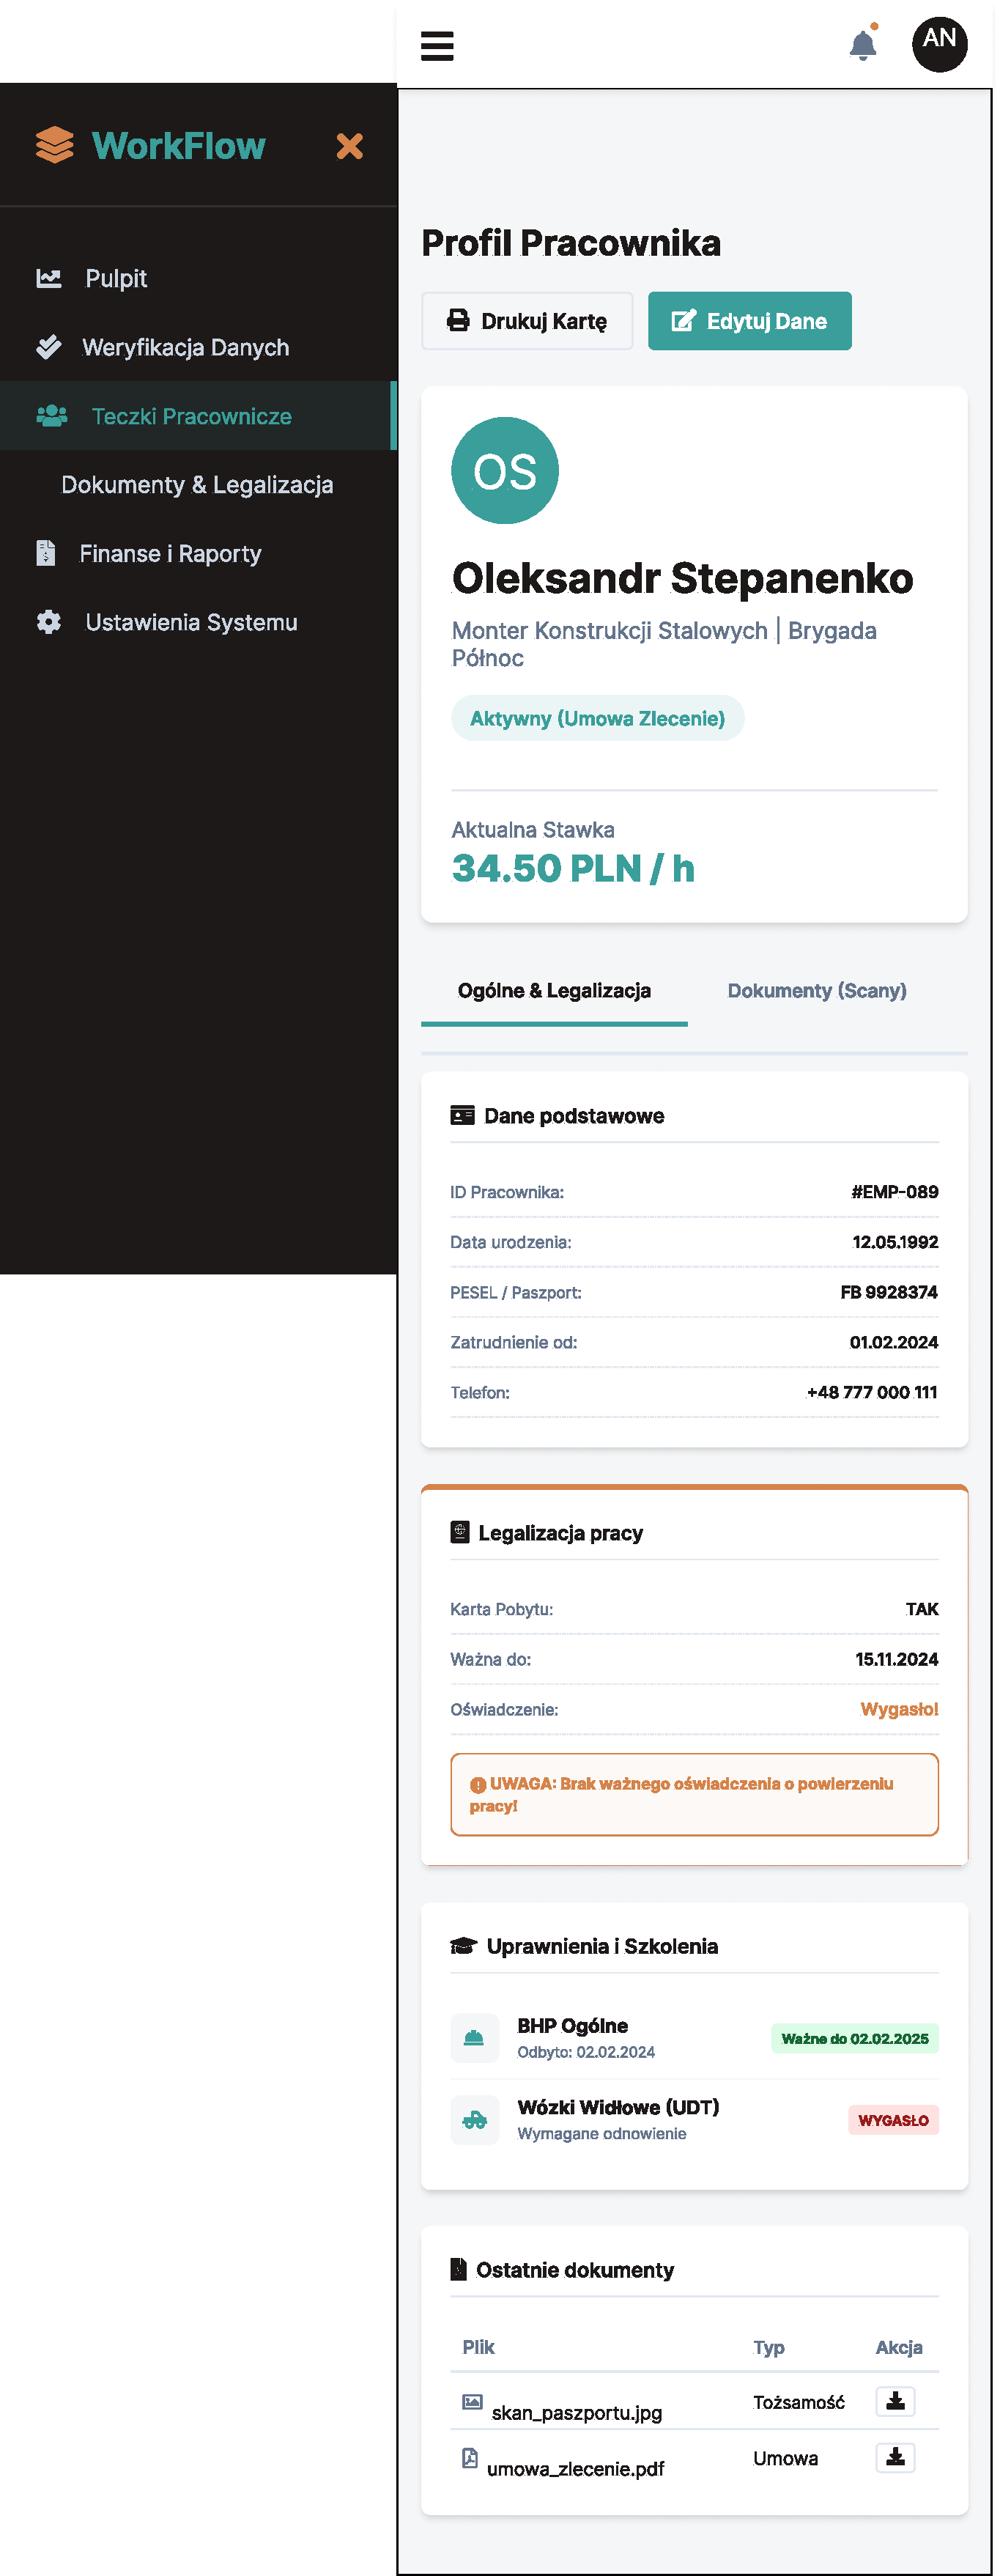
\includegraphics[width=0.35\textwidth]{rys/390w_panel.pdf}
    \caption{Widok mobilny -- profil pracownika}
    \label{fig:figma_profile_mobile}
\end{figure}

\textbf{Zakres danych prezentowanych w profilu pracownika:}
\begin{itemize}
    \item dane podstawowe, takie jak imię, nazwisko, PESEL, e-mail, rola i status aktywności,
    \item przypisanie do zakładu,
    \item identyfikator karty RFID,
    \item umowy pracownika,
    \item certyfikaty, badania i szkolenia,
    \item dokumenty powiązane z pracownikiem,
    \item nieobecności,
    \item przypisania do projektów,
    \item wpisy czasu pracy.
\end{itemize}

Profil pracownika pełni funkcję centralnego widoku kadrowego. Dzięki temu użytkownik nie musi szukać danych pracownika w wielu niezależnych miejscach. Powiązane informacje są prezentowane w jednym kontekście, co ułatwia obsługę danych kadrowych i organizacyjnych.

\subsection{Widoki tabelaryczne}

Znaczna część interfejsu systemu opiera się na widokach tabelarycznych. Dotyczy to między innymi listy pracowników, zakładów, projektów, certyfikatów, czasu pracy oraz widoków rozliczeniowych.

Widoki tabelaryczne powinny umożliwiać:
\begin{itemize}
    \item szybkie przeglądanie większej liczby rekordów,
    \item wyszukiwanie danych,
    \item filtrowanie według wybranych kryteriów,
    \item przejście do szczegółów rekordu,
    \item prezentację statusów w czytelnej formie,
    \item zachowanie spójnego układu kolumn i akcji.
\end{itemize}

W przypadku listy pracowników szczególne znaczenie mają filtry po imieniu, nazwisku, adresie e-mail, numerze PESEL, roli oraz statusie. Dla certyfikatów istotne są natomiast typ, nazwa, data ważności oraz liczba dni pozostałych do wygaśnięcia.

\subsection{Formularze}

System wykorzystuje formularze do dodawania i edycji danych. Formularze występują między innymi w modułach pracowników, zakładów, projektów, umów, certyfikatów i nieobecności.

Podczas projektowania formularzy przyjęto, że:
\begin{itemize}
    \item pola powinny być opisane w sposób jednoznaczny,
    \item dane wymagane powinny być walidowane przed zapisem,
    \item błędy powinny być prezentowane użytkownikowi w czytelny sposób,
    \item formularze powinny być możliwie krótkie i dostosowane do kontekstu,
    \item po zapisie danych użytkownik powinien otrzymać informację o rezultacie operacji.
\end{itemize}

Przykładem takiego formularza jest edycja danych pracownika, gdzie użytkownik może zaktualizować dane osobowe, adres e-mail, numer PESEL, identyfikator karty RFID, rolę oraz status aktywności.

\subsection{Tryb jasny i ciemny}

W systemie przewidziano obsługę trybu jasnego i ciemnego. Wymagało to ujednolicenia kolorów tła, tekstu, obramowań, pól formularzy oraz elementów tabelarycznych.

Obsługa dwóch motywów ma znaczenie praktyczne, ponieważ aplikacja może być używana w różnych warunkach oświetleniowych. Dodatkowo wymusza ona bardziej konsekwentne stosowanie tokenów kolorystycznych zamiast sztywnych kolorów przypisanych wyłącznie do jednego motywu.

\subsection{Znaczenie makiet dla implementacji}

Makiety stanowiły punkt wyjścia do określenia sposobu prezentacji danych oraz układu najważniejszych widoków. W trakcie implementacji część założeń została zmodyfikowana, aby lepiej dopasować interfejs do aktualnego modelu danych i dostępnych modułów.

Najważniejsze decyzje wynikające z pracy nad interfejsem to:
\begin{itemize}
    \item wykorzystanie bocznej nawigacji jako głównego sposobu poruszania się po aplikacji,
    \item centralne znaczenie profilu pracownika,
    \item prezentowanie powiązanych danych w sekcjach,
    \item stosowanie tabel dla list rekordów,
    \item oddzielenie widoków operacyjnych od widoków administracyjnych,
    \item zachowanie spójności wyglądu pomiędzy trybem jasnym i ciemnym.
\end{itemize}

W rezultacie interfejs użytkownika został podporządkowany strukturze danych oraz najważniejszym procesom systemu.